% AF benchmark vs paper baselines — legend below plot
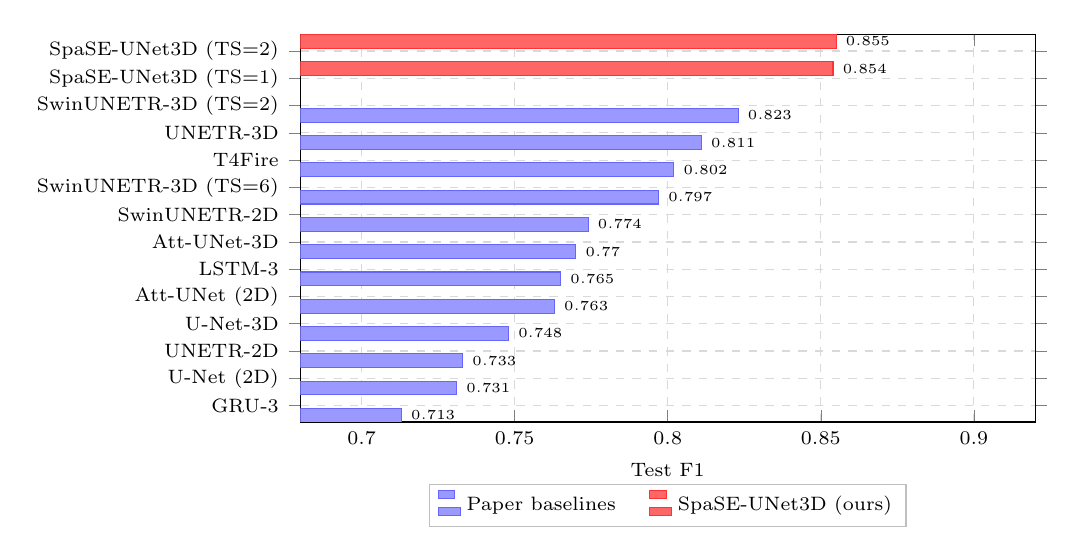
\begin{tikzpicture}
\begin{axis}[
    width=0.90\linewidth, height=6.5cm,
    xbar, bar width=5pt,
    xmin=0.68, xmax=0.92,
    enlarge y limits={abs=0.6},
    xlabel={Test F1}, ylabel={},
    grid=major, grid style={dashed, gray!30},
    tick label style={font=\scriptsize},
    xlabel style={font=\scriptsize},
    yticklabel style={font=\scriptsize},
    xtick={0.70,0.75,0.80,0.85,0.90},
    ytick={0,1,2,3,4,5,6,7,8,9,10,11,12,13},
    yticklabels={GRU-3,U-Net (2D),UNETR-2D,U-Net-3D,Att-UNet (2D),LSTM-3,Att-UNet-3D,SwinUNETR-2D,SwinUNETR-3D (TS=6),T4Fire,UNETR-3D,SwinUNETR-3D (TS=2),SpaSE-UNet3D (TS=1),SpaSE-UNet3D (TS=2)},
    nodes near coords={\pgfmathprintnumber[fixed,precision=3]{\pgfplotspointmeta}},
    nodes near coords align={horizontal},
    nodes near coords style={font=\tiny},
    legend style={font=\scriptsize, draw=gray!50,
                  at={(0.5,-0.16)}, anchor=north, legend columns=2,
                  /tikz/every even column/.append style={column sep=10pt}},
    legend cell align=left,
]
\addplot[fill=blue!40, draw=blue!60] coordinates {
    (0.713, 0) (0.731, 1) (0.733, 2) (0.748, 3) (0.763, 4) (0.765, 5)
    (0.770, 6) (0.774, 7) (0.797, 8) (0.802, 9) (0.811, 10) (0.823, 11)
};
\addlegendentry{Paper baselines}
\addplot[fill=red!60, draw=red!80] coordinates {
    (0.854, 12) (0.855, 13)
};
\addlegendentry{SpaSE-UNet3D (ours)}
\end{axis}
\end{tikzpicture}